\documentclass[]{report}

\usepackage[T1]{fontenc}
\usepackage[urw-garamond]{mathdesign}
\usepackage{garamondx}
\usepackage{amsmath, amsthm, amsfonts}
\usepackage[a4paper, total={5in, 8in}]{geometry}
\usepackage{tikz-cd} % used to draw commutative diagrams
\usepackage{graphicx}

% user defined commands go here
\newtheorem{theorem}{Theorem}[section]
\newtheorem{prop}[theorem]{Proposition}
\newtheorem{corollary}{Corollary}[theorem]
\newtheorem{lemma}[theorem]{Lemma}
\newtheorem{defn}[theorem]{Definition}
\newtheorem{examples}[theorem]{Example}
\newtheorem{exercise}[theorem]{Exercise}

\begin{document}

\title{Introduction to Commutative Algebra}
\author{Amal M}
\date{January 4, 2021}
\maketitle

\begin{abstract}

    The motivation for the study of algebraic geometry is how algebraic objects (rings of rational functions) are associated with varieties (zeros of polynomials). This subject florished during the second half of the twentieth century. Algebraic geometry allows us to study the geometry arising from algebraic objects. Core to the deeper understanding of this subject is an understanding of the subject of commutative algebra which studies commutative rings and their ideals and modules. The purpose of the present project is to gain an understanding of commutative algebra through solving exercises from Atiyah-MacDonald's book, Introduction to Commutative Algebra. The reading project comprised of the study of the theory of rings and modules, their tensor product and exact sequences of rings and modules. The project concluded with a proof of the Going-Up Theorem.

\end{abstract}

\tableofcontents
\newpage

\chapter{Introduction}

The purpose of the current project is to give an understanding 
to the reader of how commutative algebra is used to define the basic
objects of algebraic geometry. Algebraic Geometry is the study of
the geometric properties of the solution set of polynomial equations
in arbitary variables. For this purpose it is useful to confine the 
discussion to algebraically closed fields $k$ and the polynomial ring
$k[x_1,\cdots,x_n]$. We define \textit{affine n-space} over the algebraically closed field $k$ as $k^n$ and denote it by $A^n_k$.

\begin{defn} The algebraic variety \cite{vakil145} in the affine space $\mathbb{A}^n_k$ of a set $S$ of polynomials $f\in k[x_1,\cdots, x_n]$ is a subset $V(S)\subseteq \mathbb{A}^n_k$ 
    $$V(S) = \{x = (x_1,\cdots,x_n) \in \mathbb{A}^n_k : f(x) = 0 \text{ for all } f \in S\}.$$
\end{defn}

The affine variety is not the only example of a variety. The projective variety defined over projective spaces $\mathbb{P}^n_k$ is another example of an algebraic variety.

The solution set or \textit{locus} of solutions of polynomials of degree one are discrete points in $k$. But over $k^2$ the \textit{locus} are curves. For example, the solution of the elliptic curve given by the polynomial equation in $\mathbb{R}[x,y]$ in $\mathbb{R}^2$  
    $$y^2 = x^3 - 3x + 5$$
    is a curve (Fig 1.). The question then arises: \textit{what does the solution set of a set of polynomials in $k^3$ look like? What about $k^n$?} This is same asking the question: \textit{what does an affine algebraic variety in $A^n_k$ look like?} We may go further by demanding: \textit{what is the topology of the affine algebraic variety?} (The answer is called the \textit{Zariski Topology}, which we shall get to in due time.)

    Once we have an affine algebraic variety we may define functions on them and we may define functions from one algebraic variety to another. That is we start to do the usual mathematical \textit{shtick} on affine varieties.

    To answer the proposed questions we need to know the properties of an affine algebraic varieties. For example: \textit{what is so algebraic about an affine algebraic variety?} The answer is that we may consider every \textit{affine algebraic variety} to be some \textit{finitely generated nilpotent-free $k$-algebra $A$}. To know what each of these terms means we first need some commutative algebra. The purpose of this article is to explain these terms and give a brief introduction to Algebraic Geometry.


\begin{figure}
  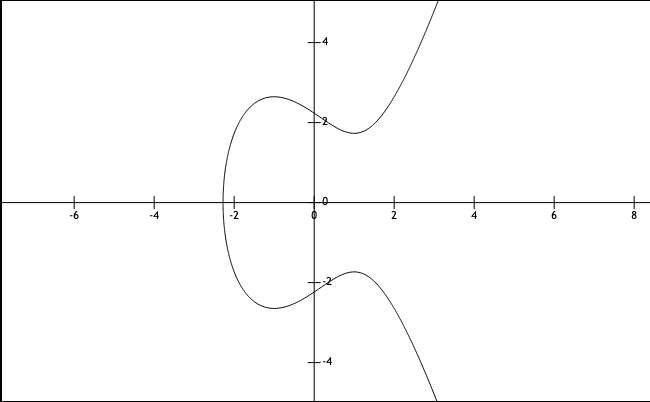
\includegraphics[width=\linewidth]{img/ell_curv1.png}
  \caption{Fig 1.}
  \label{fig:ell_curv1}
\end{figure}


\section{Prime Spectrum}
\section{Zariski Topology}
\section{Irreducible Spaces}
\section{Affine Algebraic Varieties}


\chapter{Tensor Product and Direct Limits}
\section{Tensor Product}
\section{Flatness}
\section{Direct Limit}

\chapter{Sheaf and Presheaf}
\section{Support}
\section{Presheaf}
\section{Sheaf}
\section{Constructible Topology}
\section{Absolute Flatness}

\begin{thebibliography}{9}

\bibitem{vakil145}
    Ravi Vakil,
    \textit{Math 145: Algebraic Geometry}
\end{thebibliography}

\end{document}
